\section{Примеры использования}

Интеллектуальная система машинного обучения была разработана с целью поддержки полного цикла исследования поведения нейросетевых моделей, включая этапы создания данных, обучения классификатора, анализа и интерпретации результатов. Ниже приведены ключевые сценарии использования системы, иллюстрирующие её функциональные возможности.

%%%%%%%%%%%%%%%%%%%%%%%%%%%%%%%%%%%%%%%%%%%%%%%%%%%%%%%%%%%%%%%%%%%%%%%%%%%%%%%%%%%%%%%%%%%%%%%%%%%%%%%%%%%%%%%
\subsection{Бинарная классификация}
Для проверки способности модели к нелинейной аппроксимации границ принятия решений решается задача классификации двух переплетённых спиралей (рисунок~\cref{fig:vis_binary_classification}). В системе предусмотрена генерация соответствующего набора данных и обучение модели с возможностью пошагового отображения изменения решения по мере выполнения эпохи градиентного спуска. Интеллектуальная система машинного обучения позволяет наблюдать как локальные ошибки, так и итоговую зону классификации, что особенно полезно при выборе архитектуры сети и прочих гиперпараметров.

\begin{figure}[ht]
    \centerfloat{
        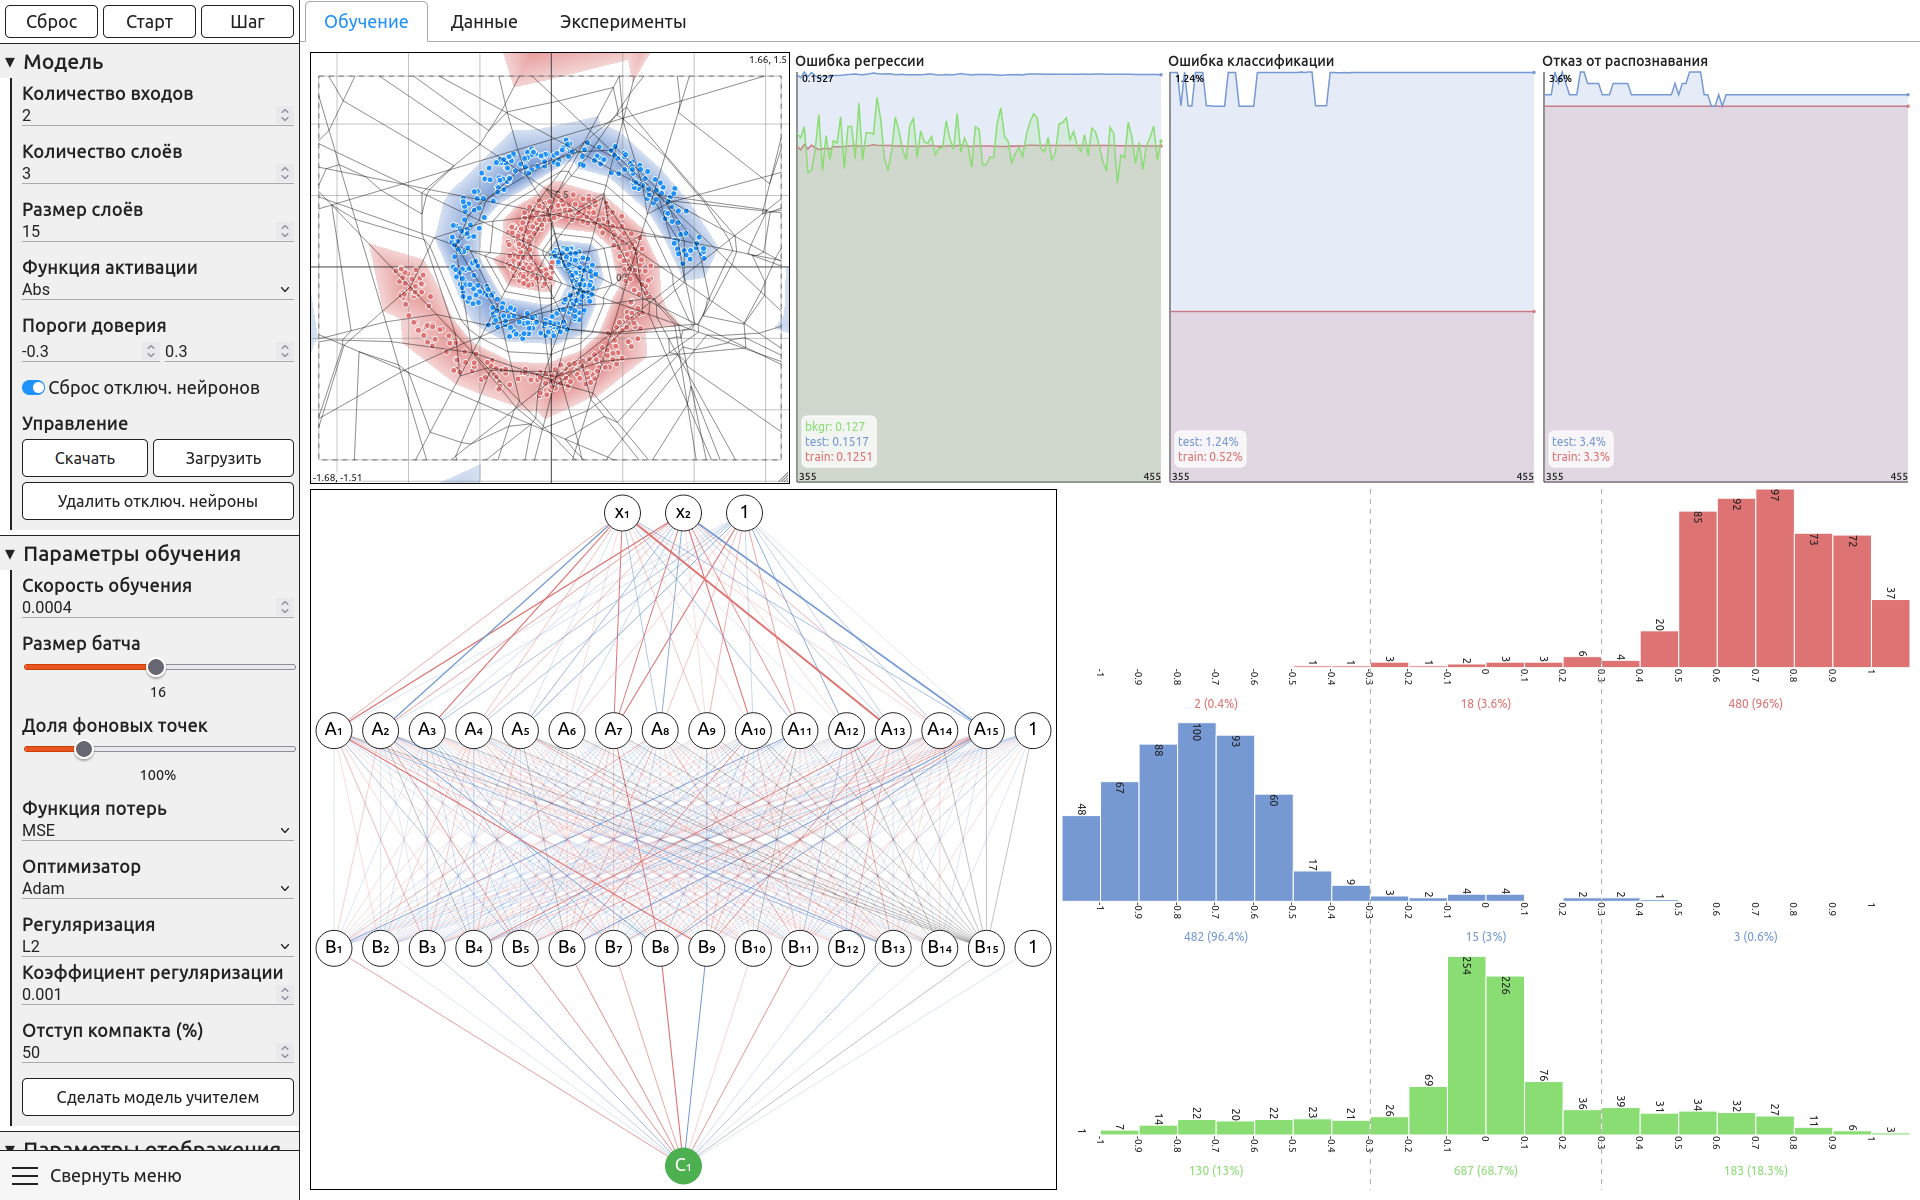
\includegraphics[width=0.9\linewidth]{Dissertation/images/ch4/usage/binary_classification.png}
    }
    \caption{Пример выполнения бинарной классификации}
    \label{fig:vis_binary_classification}
\end{figure}

%%%%%%%%%%%%%%%%%%%%%%%%%%%%%%%%%%%%%%%%%%%%%%%%%%%%%%%%%%%%%%%%%%%%%%%%%%%%%%%%%%%%%%%%%%%%%%%%%%%%%%%%%%%%%%%
\subsection{Унарная классификация}
Режим унарной классификации допускает обучение модели только по положительным примерам, дополненным фоновыми объектами (рисунок~\cref{fig:vis_unary_classification}). В качестве примера используется одна из спиралей из предыдущего эксперимента. Пользователь может задать уровень порога \(\beta\), визуализировать полученную область принятия положительного класса, а также проследить, каким образом меняется зона отказа при варьировании параметров. Данный сценарий позволяет исследовать свойство доверия, характерное для унарных моделей.

\begin{figure}[ht]
    \centerfloat{
        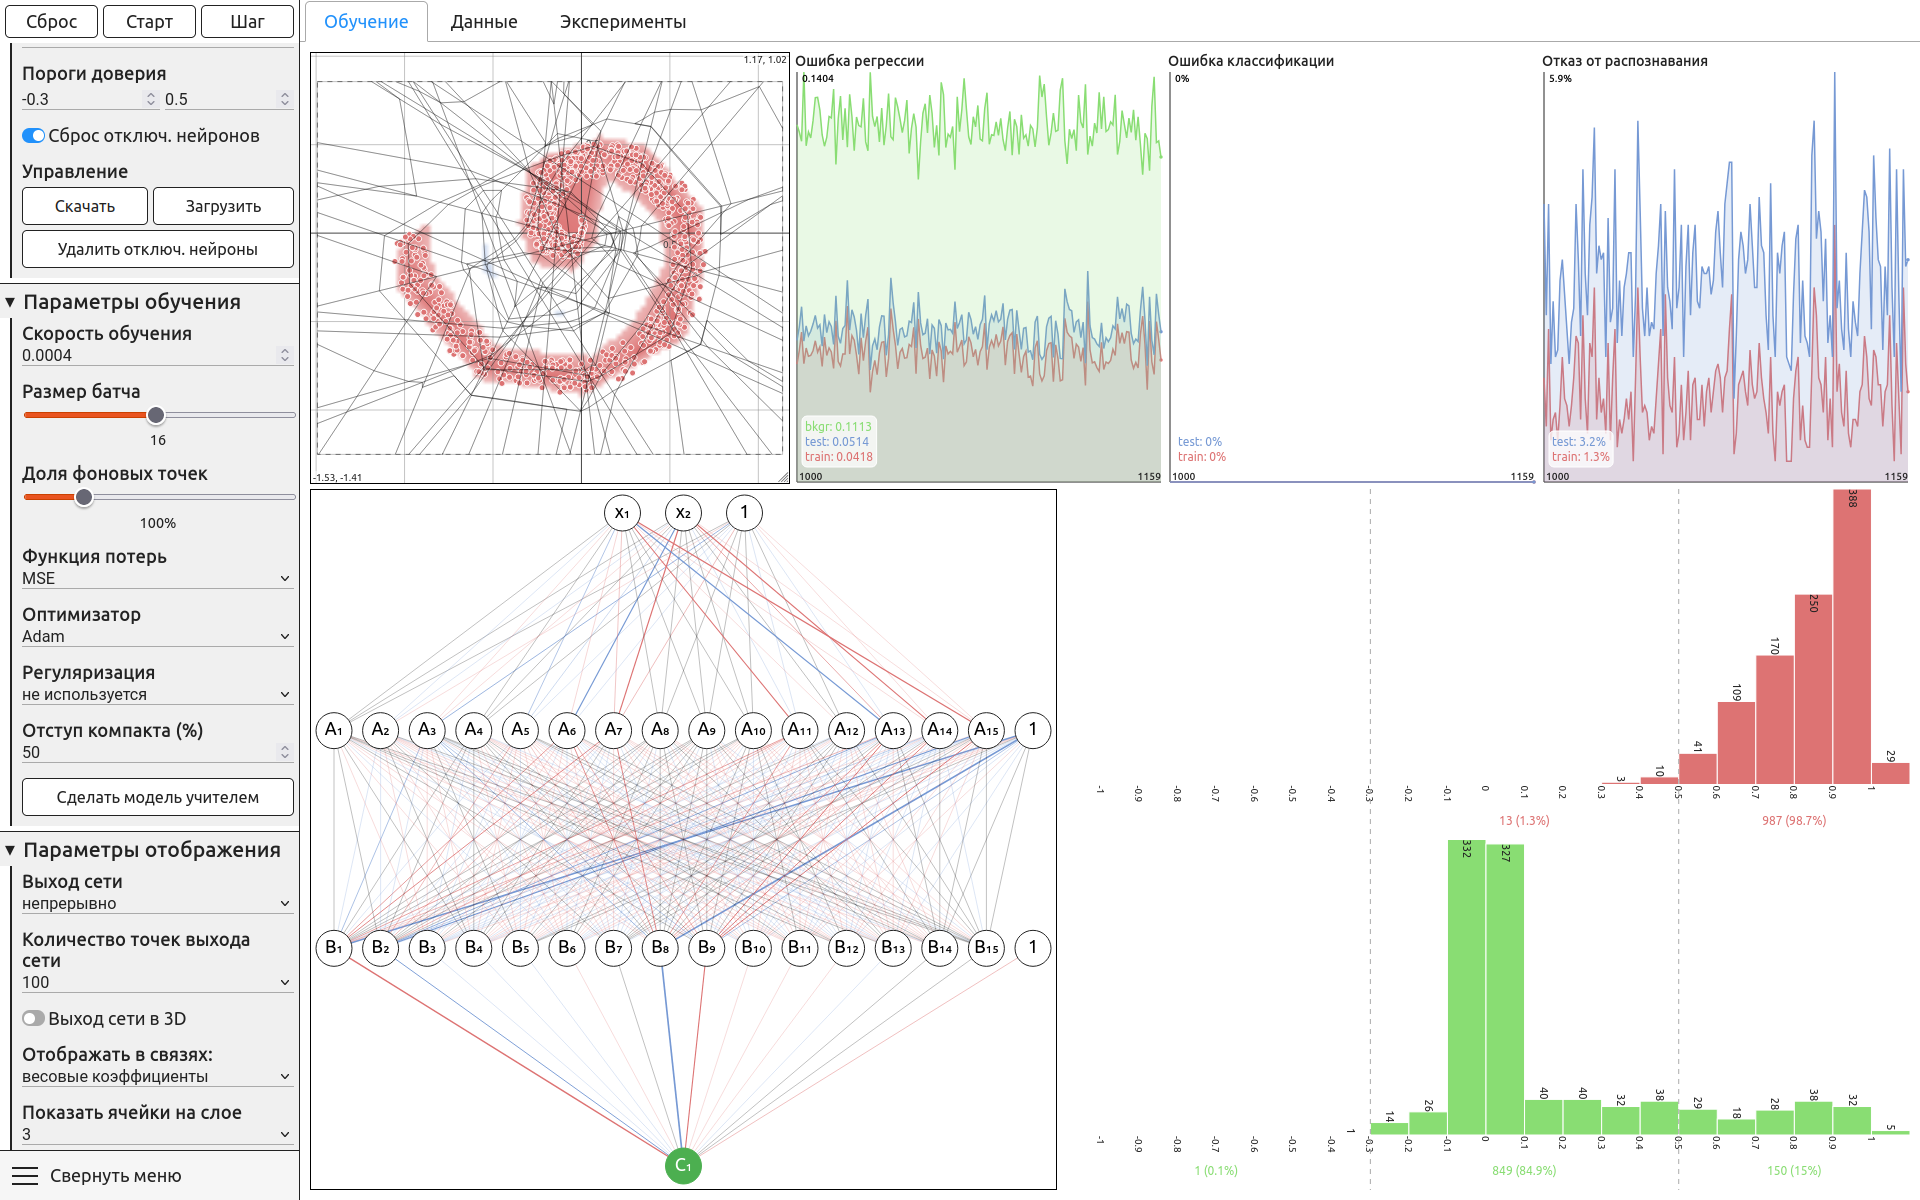
\includegraphics[width=0.9\linewidth]{Dissertation/images/ch4/usage/unary_classification.png}
    }
    \caption{Пример выполнения унарной классификации}
    \label{fig:vis_unary_classification}
\end{figure}

%%%%%%%%%%%%%%%%%%%%%%%%%%%%%%%%%%%%%%%%%%%%%%%%%%%%%%%%%%%%%%%%%%%%%%%%%%%%%%%%%%%%%%%%%%%%%%%%%%%%%%%%%%%%%%%
\subsection{Создание синтетических данных}
Одной из оригинальных функций системы является реализация метода синтетической генерации данных на основе репродукции, предложенного в рамках диссертационного исследования. Данный метод позволяет строить приближённую аппроксимацию распределения положительного класса в пространстве признаков, используя предварительно обученную унарную модель (рисунок~\cref{fig:vis_synthetic_data}).

\begin{figure}[ht]
    \centerfloat{
        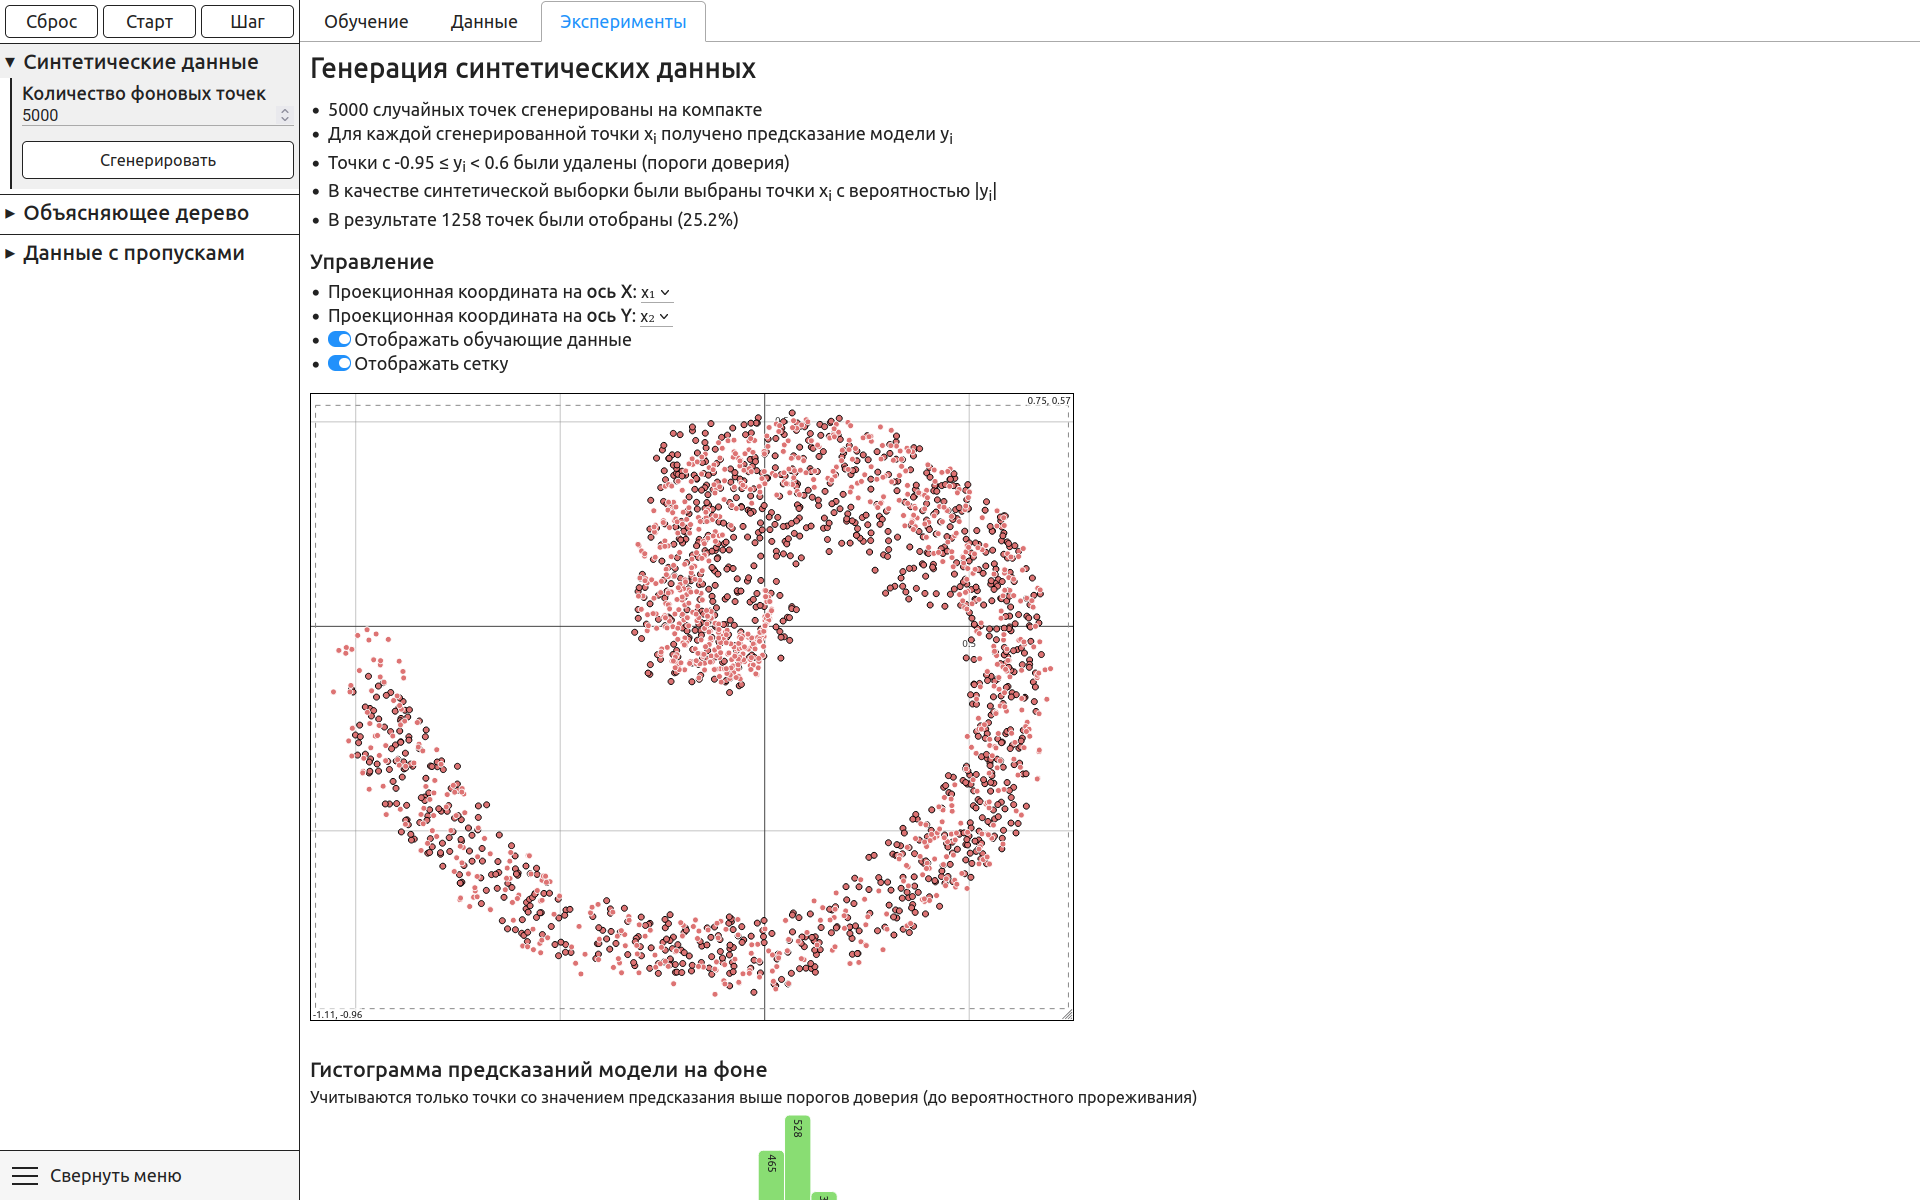
\includegraphics[width=0.9\linewidth]{Dissertation/images/ch4/usage/synthetic_data.png}
    }
    \caption{Пример построения синтетических данных}
    \label{fig:vis_synthetic_data}
\end{figure}

Пользователь может интерактивно варьировать пороговое значение, наблюдать за плотностью отобранных объектов, а также визуализировать геометрию полученного множества. Данная возможность особенно важна при построении новых обучающих выборок, моделировании редких классов и оценке обобщающей способности модели на слабо покрытых областях признакового пространства.

%%%%%%%%%%%%%%%%%%%%%%%%%%%%%%%%%%%%%%%%%%%%%%%%%%%%%%%%%%%%%%%%%%%%%%%%%%%%%%%%%%%%%%%%%%%%%%%%%%%%%%%%%%%%%%%
\subsection{Построение объясняющего дерева решений}
Одним из компонентов системы является модуль построения объясняющего дерева решений, предназначенного для геометрического описания поведения и интерпретации решения обученного персептрона (рисунок~\cref{fig:vis_extree}). Пользователь может выбрать интересующую ячейку и подробно изучить как её содержимое, так и геометрию пространства. Это позволяет проводить интерпретацию решения в выбранной области и служит средством повышения доверия к результатам классификации.

\begin{figure}[ht]
    \centerfloat{
        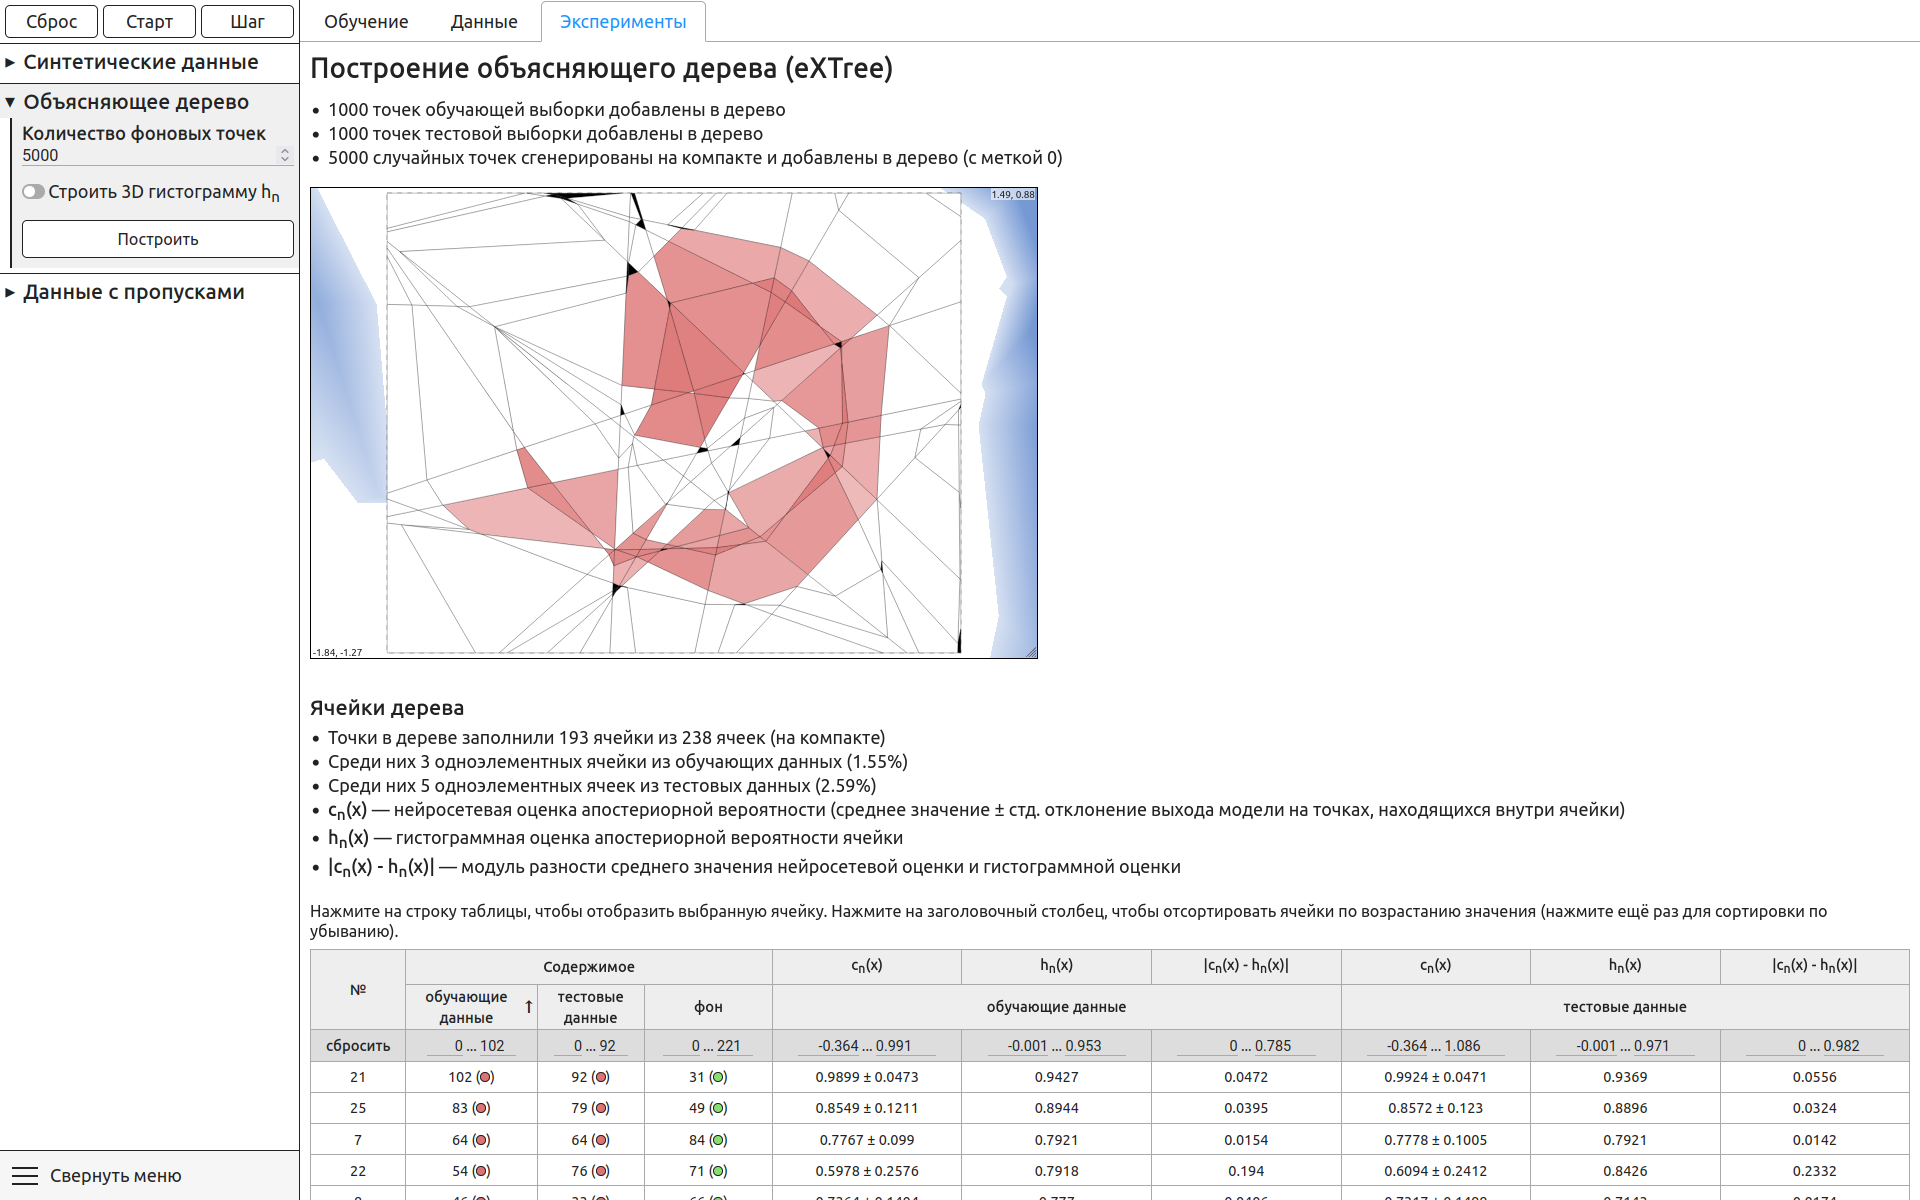
\includegraphics[width=0.9\linewidth]{Dissertation/images/ch4/usage/extree.png}
    }
    \caption{Пример работы с объясняющим деревом}
    \label{fig:vis_extree}
\end{figure}
